% Ensure included PDFs (banners) with newer versions embed without warnings
\pdfminorversion=7
\documentclass[aspectratio=169]{beamer}

\makeatletter
% Make LaTeX find theme .sty files in Template
\def\input@path{{../Template/}}
\makeatother
\usepackage{graphicx}
% Make graphics (including banner PDFs) resolvable without TEXINPUTS
\graphicspath{{../Template/}{../Template/banners/}{../../Common_Images/}}

%================================================================%
% Theme and Package Setup
%================================================================%
\usetheme{ucl}
\setbeamercolor{banner}{bg=darkpurple}

% Navigation and Footer
\setbeamertemplate{navigation symbols}{\vspace{-2ex}}
\setbeamertemplate{footline}[author title date]
\setbeamertemplate{slide counter}[framenumber/totalframenumber]

\usepackage[utf8]{inputenc}
\usepackage[british]{babel} % British spelling
\usepackage{amsmath, amssymb, amsthm}
\usepackage{graphicx}
\usepackage{tikz}
\usetikzlibrary{calc, positioning, arrows.meta, shapes.geometric, trees, backgrounds, shapes.misc, graphs, quotes, shadows, fit, patterns} 
\usepackage{pgfplots}
\pgfplotsset{compat=1.17}
\usefonttheme{professionalfonts}
\usepackage{eulervm}
\usepackage{listings}
\usepackage{algorithm}
\usepackage{algpseudocode}
\usepackage{xcolor}
\usepackage{subcaption}

% Define custom colours
\makeatletter
\@ifundefined{color@stone}{%
    \definecolor{stone}{gray}{0.95}%
}{}
\makeatother
\definecolor{darkgreen}{rgb}{0.0, 0.5, 0.0}
\definecolor{uclblue}{cmyk}{1,0.24,0,0.64}
\definecolor{uclred}{cmyk}{0,1,0.62,0}
\definecolor{uclpurple}{cmyk}{0.32,0.42,0,0.55}
\definecolor{uclorange}{cmyk}{0,0.45,0.91,0}

% Semantic colours from Lecture 1
\definecolor{liftblue}{RGB}{44, 123, 182}
\definecolor{liftorange}{RGB}{253, 141, 60}
\definecolor{liftgreen}{RGB}{26, 150, 65}
\definecolor{liftred}{RGB}{215, 25, 28}

\newcommand{\standard}[1]{{\color{liftblue}#1}}
\newcommand{\relaxation}[1]{{\color{liftorange}#1}}
\newcommand{\bregman}[1]{{\color{liftgreen}#1}}
\newcommand{\failure}[1]{{\color{liftred}#1}}

% TikZ Styles
\tikzset{
    statebox/.style={rectangle, rounded corners, draw=black, thick, fill=stone, minimum width=1.2cm, minimum height=0.6cm, align=center},
    standardarrow/.style={-{Stealth[scale=1.2]}, thick},
    backarrow/.style={-{Stealth[scale=1.2]}, thick, dashed, draw=liftred},
    relaxarrow/.style={-{Stealth[scale=1.2]}, thick, draw=liftorange},
    bregmanarrow/.style={-{Stealth[scale=1.2]}, thick, draw=liftgreen},
    note/.style={font=\scriptsize, align=center}
}

\setbeamercovered{transparent}

% Define theoremblock
\makeatletter
\newenvironment<>{theoremblock}[1]{%
    \begin{block}#2{#1}%
}{\end{block}}
\makeatother

% Section divider slides
\AtBeginSection[]{
  \begin{frame}
    \frametitle{\textbf{\Large\insertsectionhead}}
    \begin{center}
        \huge\textbf{\insertsectionhead}
    \end{center}
  \end{frame}
}

% Maths Macros
\newcommand{\U}{\mathcal{U}}
\newcommand{\V}{\mathcal{V}}
\newcommand{\Z}{\mathcal{Z}}
\newcommand{\R}{\mathbb{R}}
\newcommand{\E}{\mathbb{E}}
\newcommand{\ip}[2]{\langle #1, #2 \rangle}
\newcommand{\norm}[1]{\| #1 \|}
\DeclareMathOperator*{\argmin}{argmin}
\DeclareMathOperator{\prox}{prox}
\DeclareMathOperator{\dom}{dom}
\DeclareMathOperator{\supremum}{sup}
\DeclareMathOperator{\sign}{sign}

\title{Lifted Neural Network Training}
\subtitle{Part 2: Unified Architectures and Computational Optimisation Strategies}
\author[Martin Benning (University College London)]{Martin Benning}
\date[COMP0263]{COMP0263 -- Solving Inverse Problems with Data-Driven Models \\[1cm] 17th March 2026}
\institute[]{University College London}

\begin{document}

% --- Title Frame ---
\begin{frame}
  \titlepage
\end{frame}

% --- Outline ---
\begin{frame}{Lecture Overview}
    \tableofcontents
\end{frame}

% ==============================================================================
\section{The Unified Block-Operator Framework}
% ==============================================================================

\begin{frame}{Recap \& Motivation}
    In the previous lecture, we established the \textbf{Lifted Bregman framework} as a principled method for bypassing sequential gradient bottlenecks and handling non-smooth activations natively.
    
    \vspace{1em}
    \textbf{The core idea:} We decoupled the nonlinearities using auxiliary variables and penalised consistency with a Bregman/Fenchel-Young gap.
    
    \vspace{1em}
    In this lecture we will see that this is not just useful for perceptrons or MLPs. We can encapsulate many diverse neural models under a \textbf{single unifying framework}.
\end{frame}

\begin{frame}{A Unified System of Equations}
    Diverse neural models can be represented via a unified block-operator framework \cite{wang2025unified}. For an input vector $y$, the predicted output $N(y)$ produced by the network is determined by
    \begin{theoremblock}{Unified Architecture}
        \vspace{-0.15cm}
    $$N(y) = A u + d$$
    $$M u = V z$$
    $$z = \sigma(W u + b)$$
    \end{theoremblock}
    \begin{itemize}
        \item $u$: Stacked collection of hidden/pre-activation states across all layers.
        \item $z$: Corresponding post-activation variables.
        \item $A, M, V, W$: Block-linear operators.
        \item $b, d$: Bias terms.
    \end{itemize}
\end{frame}

\begin{frame}{Deconstructing the Operators}
    What do these operators physically represent in a neural network?
    
    \begin{itemize}
        \item \textbf{Readout ($A, d$):} $A$ (usually) extracts the final output from the stacked state $u$, applying any final linear transformation and adding bias $d$.
        \item \textbf{Layer Coupling ($M, V$):} The pair $(M,V)$ encodes how neighbouring blocks/layers are structurally connected (e.g., direct feed-forward, residual shortcuts aka skip connections).
        \item \textbf{Affine Mapping ($W, b$):} $W$ collects the weight matrices to which the non-linearity $\sigma$ is applied, with bias $b$.
    \end{itemize}
    
    
\end{frame}

\begin{frame}{The Generic Lifted Objective}
    For training samples $\{(x^i,y^i)\}_{i=1}^s$, this architecture induces a generic objective:
    
    \begin{theoremblock}{Unified Lifted Objective}
    $$\min_{\mathbf{\Theta},\{u^i,z^i\}_{i=1}^s} \frac{1}{s}\sum_{i=1}^s \Big[ 
        \underbrace{\ell\left(y^i, A u^i + d\right)}_{\text{\standard{Loss}}} + 
        \underbrace{\mathcal{C}\left(Mu^i, Vz^i\right)}_{\text{\failure{Coupling}}} + 
        \underbrace{\mathcal{D}_{\sigma}\left(z^i, Wu^i + b\right)}_{\text{\bregman{Activation}}} 
    \Big]$$
    \end{theoremblock}
    
    \begin{itemize}
        \item $\mathbf{\Theta}$: Learnable entries of the block operators ($W, A, V, M$) and biases.
        \item \failure{$\mathcal{C}$}: Penalises violations of the architectural coupling $Mu=Vz$.
        \item \bregman{$\mathcal{D}_{\sigma}$}: Penalises violations of the activation relation $z=\sigma(Wu+b)$.
    \end{itemize}
\end{frame}

\begin{frame}{The Paradigm Shift: It's Just the Penalty}
    \begin{alertblock}{Key Theoretical Takeaway}
        Once this unified system is written down, the difference between conventional back-propagation and lifted training is entirely encoded by the \textbf{choice of penalty terms}, not the architecture itself!
    \end{alertblock}
    
    \failure{\textbf{Conventional Training (Hard Constraints):}}
    \[
        \failure{\mathcal{C}(a,a') = \chi_{\{0\}}(a-a') \, , \qquad \mathcal{D}_{\sigma}(z,v) = \chi_{\{0\}}\!\left(z-\sigma(v)\right)}
    \]
    
    \bregman{\textbf{Lifted Bregman Training (Soft Convex Relaxations):}}
    
    Choose \bregman{$\mathcal{D}_{\sigma}$} as the layer-wise Bregman loss \bregman{$B_{\Psi}$}. This transforms the non-convex constraints into a block-separable, bi-convex penalty structure!
\end{frame}

% ==============================================================================
\section{Formulating Standard Architectures}
% ==============================================================================

\begin{frame}{1. Single-Layer Perceptrons}
    To write a perceptron $N(x) = \sigma(w^\top x + b)$ in our unified form, we introduce an auxiliary scalar $\zeta$ and stack our variables: $u=(x,\zeta)^\top$.
    
    \vspace{1em}
    We assign the operators as follows:
    $$W = \begin{pmatrix} w^\top & 0 \end{pmatrix} \, , \quad M=A=\begin{pmatrix}0 & 1\end{pmatrix} \, , \quad V=1 \, , \quad d=0$$
    
    \vspace{1em}
    \textbf{Verification:}
    \begin{itemize}
        \item Coupling: $Mu = Vz \implies \zeta = z$
        \item Activation: $z = \sigma(Wu+b) \implies z = \sigma(w^\top x + b)$
        \item Readout: $N(x) = Au = \zeta = \sigma(w^\top x + b)$
    \end{itemize}
\end{frame}

\begin{frame}{2. Shallow Neural Networks}
    For a shallow network $N(x)=\sum_{j=1}^{J} c_j\,\sigma_j(w_j^\top x+b_j)$, we introduce auxiliary variables $\zeta_1,\ldots,\zeta_J$ and define the state vector $u=(x,\zeta_1,\ldots,\zeta_J)^\top$ and activation variables $z=(z_1,\ldots,z_J)^\top$.
    
    \vspace{1em}
    The readout and coupling become:
    $$A=\begin{pmatrix}0_{1\times M}&c_1&\cdots&c_J\end{pmatrix} \, , \quad M=\begin{pmatrix}0_{J\times M}&I_J\end{pmatrix} \, , \quad V=I_J$$
    
    And the stacked weight matrix acts on the input part of $u$:
    $$W=\begin{pmatrix} w_1^\top & 0 & \cdots & 0\\ \vdots & \vdots & \ddots & \vdots\\ w_J^\top & 0 & \cdots & 0 \end{pmatrix}$$
\end{frame}

\begin{frame}{3. Multi-Layer Perceptrons (MLPs)}
    \begin{columns}[T,onlytextwidth]
        \column{0.55\textwidth}
        For an $L$-layer MLP, the forward pass is $x^l = \sigma_l(W_l x^{l-1} + b_l)$.
        We stack everything: $u = \bigl((x^0)^\top, \ldots, (x^L)^\top\bigr)^\top$ and $z = \bigl((z^1)^\top, \ldots, (z^L)^\top\bigr)^\top$.
        
        %\vspace{1em}
        The weight matrix $W$ is \textbf{block sub-diagonal}:
        $$W = \begin{pmatrix} W_1 & 0 & 0 & \cdots & 0 \\ 0 & W_2 & 0 & \cdots & 0 \\ \vdots & & \ddots & & \vdots \\ 0 & \cdots & & W_L & 0 \end{pmatrix}$$

        Applying $Wu+b$ assembles $(W_1 x^0 + b_1, \ldots)^\top$ in one operation.
        
        \column{0.45\textwidth}
        \centering
        \vspace{1em}
        \begin{tikzpicture}[scale=0.9, transform shape]
            \node[statebox] (x0) at (0,3) {$x^0$};
            \node[statebox] (x1) at (0,1.5) {$x^1$};
            \node (dots) at (0,0.5) {$\vdots$};
            \node[statebox] (xL) at (0,-0.5) {$x^L$};
            
            \draw[standardarrow] (x0) -- node[right,note] {$W_1, \sigma_1$} (x1);
            \draw[standardarrow] (x1) -- node[right,note] {$W_2, \sigma_2$} (dots);
            \draw[standardarrow] (dots) -- node[right,note] {$W_L, \sigma_L$} (xL);
            
            % Highlight the block diagonal nature
            \draw[thick, liftblue, rounded corners, dashed] (-1.5, 0.8) rectangle (1.5, 3.5);
            \node[liftblue, note] at (2.2, 2.25) {$W$ acts on \\ previous \\ layer};
        \end{tikzpicture}
    \end{columns}
\end{frame}

\begin{frame}{Multi-Layer Perceptrons (Continued)}
    The coupling matrix $M$ acts as a \textbf{block identity shift}, extracting the post-activation states $(x^1, \ldots, x^L)$ from $u$:
    
    $$M = \begin{pmatrix} 0 & I_{N_1} & 0 & \cdots & 0 \\ 0 & 0 & I_{N_2} & \cdots & 0 \\ \vdots & \vdots & & \ddots & \vdots \\ 0 & 0 & \cdots & & I_{N_L} \end{pmatrix}$$
    
    
    
    Since $V=I$, the coupling $Mu = Vz$ simply asserts $z^l = x^l$ for all layers simultaneously. The output map $A$ zeroes all but the final block $x^L$ and applies the readout weights $K$.
\end{frame}

\begin{frame}{4. Residual Networks (ResNets)}
    \begin{columns}[T,onlytextwidth]
        \column{0.55\textwidth}
        For an $L$-block ResNet, the residual update is $x^l = x^{l-1} + h_l V_l \sigma_l(W_l x^{l-1} + b_l)$. 
        
        To enforce this skip-connection structure, $M$ becomes a \textbf{block first-difference operator}:
        $$M = \begin{pmatrix} -I & I & 0 & \cdots & 0 \\ 0 & -I & I & \cdots & 0 \\ \vdots & & \ddots & \ddots & \vdots \\ 0 & \cdots & & -I & I \end{pmatrix}$$
        
        $V$ becomes a block-diagonal matrix holding the scaled residual weights $h_l V_l$. 

        \column{0.45\textwidth}
        \centering
        \textbf{Skip Connection ($M$)} \\
        \vspace{1em}
        \begin{tikzpicture}[scale=0.9, transform shape]
            \node[statebox] (xprev) at (0,2.5) {$x^{l-1}$};
            \node[statebox, minimum width=2.5cm] (F) at (0,1) {$h_l V_l \sigma_l(W_l \cdot + b_l)$};
            \node[statebox] (xl) at (0,-1.0) {$x^l$};
            \node[circle, draw, thick, inner sep=1pt] (plus) at (0, 0.25) {$+$};

            \draw[standardarrow] (xprev) -- (F);
            \draw[standardarrow] (F) -- (plus);
            \draw[standardarrow] (plus) -- (xl);
            
            % Skip connection
            \draw[thick, liftblue, -{Stealth[scale=1.2]}] (xprev.west) -- ++(-1.2,0) |- node[left,pos=0.25] {Identity ($I$)} (plus.west);
        \end{tikzpicture}
    \end{columns}
    
    Thus, $Mu = Vz \implies \standard{x^l - x^{l-1}} = h_l V_l z^l$, recovering forward Euler discr. of ODE \cite{benning2019deep}
\end{frame}

\begin{frame}{5. Proximal Neural Networks (LISTA)}
    PNNs unroll algorithms like ISTA for $J$ iterations: $\alpha_j = \mathcal{S}_{\gamma_j\lambda_j}\!\bigl(\widetilde{W}_j\,\alpha_{j-1} + \tilde{b}_j\bigr)$.
    
    \vspace{1em}
    Here, the activation function $\sigma$ is composed of soft-thresholding operators. $W$ holds the ISTA step matrices $\widetilde{W}_j = I - \gamma_j \Phi_j^\top H^\top H \Phi_j$, and the bias $b$ provides the data-driven forcing.
    
    \begin{alertblock}{The Perfect Fit for Bregman}
        PNNs are central to the lifted Bregman setting because soft-thresholding satisfies the proximal structure $\operatorname{prox}_{\gamma_j\lambda_j\|\cdot\|_1}$ \textit{by construction}. The Bregman loss applies natively to every unrolled iterate update!
    \end{alertblock}
\end{frame}

% ==============================================================================
\section{Optimisation Algorithms for Lifted Training}
% ==============================================================================

\begin{frame}{Solving the Unified Objective}
    How do we actually train this? By lifting the network, we trade a deeply nested, highly non-convex structure for a larger, but \textbf{block-separable} optimisation problem.
    
    \vspace{1em}
    Writing the total objective as $\mathcal{J}(\mathbf{\Theta},\mathbf{X})$, a basic deterministic \textbf{Block-Coordinate Descent (BCD)} strategy alternates between updating parameters and auxiliary states:
    
    \begin{theoremblock}{Global BCD Updates}
    $$\mathbf{\Theta}^{k+1} \in \argmin_{\mathbf{\Theta}} \mathcal{J}(\mathbf{\Theta},\mathbf{X}^k)$$
    $$\mathbf{X}^{k+1} \in \argmin_{\mathbf{X}} \mathcal{J}(\mathbf{\Theta}^{k+1},\mathbf{X})$$
    \end{theoremblock}
\end{frame}

\begin{frame}{Inexact Block Updates}
    Because exact minimisation of the global blocks is often too computationally expensive, we rely on \textbf{inexact block updates}.
    
    \vspace{1em}
    For MAC, Fenchel, and Bregman-type relaxations, the layer-wise subproblems are \textbf{convex} in each block.
    
    \begin{itemize}
        \item We can apply \textbf{Proximal Gradient Descent} (PGD) to parameter blocks and auxiliary-variable blocks.
        \item Whenever a smooth data-fit term is coupled with non-smooth regularisation (e.g., $\ell_1$ sparsity), we deploy ISTA-type updates locally at the layer level.
    \end{itemize}
\end{frame}

\begin{frame}{Scaling Up: Mini-Batching and ISGM}
    For large datasets, deterministic BCD over the entire dataset is infeasible. Instead, we use mini-batching.
    
    \vspace{1em}
    A particularly useful instance is the \textbf{Implicit Stochastic Gradient Method (ISGM)}:
    \begin{itemize}
        \item At each stochastic step, one forms a proximally regularised local subproblem for the active batch.
        \item This inner subproblem is approximated by a small number of inner BCD/proximal-gradient sweeps.
    \end{itemize}
    
    \vspace{1em}
    \textbf{Advantages:} Compared to explicit SGD back-propagation, ISGM is far less sensitive to learning-rate choices and only requires storing auxiliary variables for the currently active batch in memory.
\end{frame}

\begin{frame}{A Flexible Hierarchy of Solvers}
    Lifted training is best viewed as a \textit{structured optimisation framework} rather than one fixed update rule. 
    
    \vspace{1em}
    We can naturally refine this framework using tools from earlier in the course:
    \begin{itemize}
        \item \textbf{Acceleration:} Nesterov or Heavyball momentum can be seamlessly added to the gradient-type block updates.
        \item \textbf{Adaptivity:} Adam-style preconditioning can be applied to both parameter and auxiliary blocks to handle ill-conditioned landscapes.
    \end{itemize}
\end{frame}

% ==============================================================================
\section{Practical Training Applications}
% ==============================================================================

\begin{frame}{Why Explicit Auxiliary States Matter}
    In practice, the lifted formulation is most powerful when one wants to \textbf{regularise hidden variables directly}.
    
    \vspace{1em}
    Because the auxiliary states (the post-activations $x_l$) are explicit optimisation variables in the BCD loop, we can impose structure-inducing penalties locally without breaking the chain rule. 
    
    \vspace{1em}
    Let's look at \textbf{Sparse Autoencoders} as a prime example.
\end{frame}

\begin{frame}{Sparse Autoencoders}
    Consider a lifted sparse autoencoder with even depth $L$ and a central "code" layer index $m:=L/2$. We want the latent code $x_m^i$ to be highly sparse.
    
    \begin{theoremblock}{Sparse Autoencoder Lifted Objective}
    $$\min_{\mathbf{\Theta},\mathbf{X}}\; \frac{1}{s}\sum_{i=1}^{s} \left[ \underbrace{\frac12\|x_0^i-x_L^i\|_2^2}_{\text{Reconstruction}} + \underbrace{\alpha\|x_m^i\|_1}_{\text{Sparsity Penalty}} + \underbrace{\sum_{l=1}^{L-1} \lambda_l B_{\Psi_l}\!\left(x_l^i, f(x_{l-1}^i,\Theta_l)\right)}_{\text{Bregman Consistency}} \right]$$
    \end{theoremblock}
    
    For \textbf{Denoising} autoencoders, we simply replace the clean inputs in the encoder with corrupted samples $\tilde{x}_0^i$ while reconstructing the clean target $x_0^i$.
\end{frame}

\begin{frame}{Visualising Training Trajectories}
    \only<1>{Lifted Bregman training can rapidly reduce the sparse-autoencoder objective while sustaining high code sparsity, producing high-quality reconstructions on validation data.}
    
    \vspace{0.5em}
    \begin{columns}[T,onlytextwidth]
        \column{0.48\textwidth}
        \centering
        \textbf{Objective \& Sparsity Drop} \\
        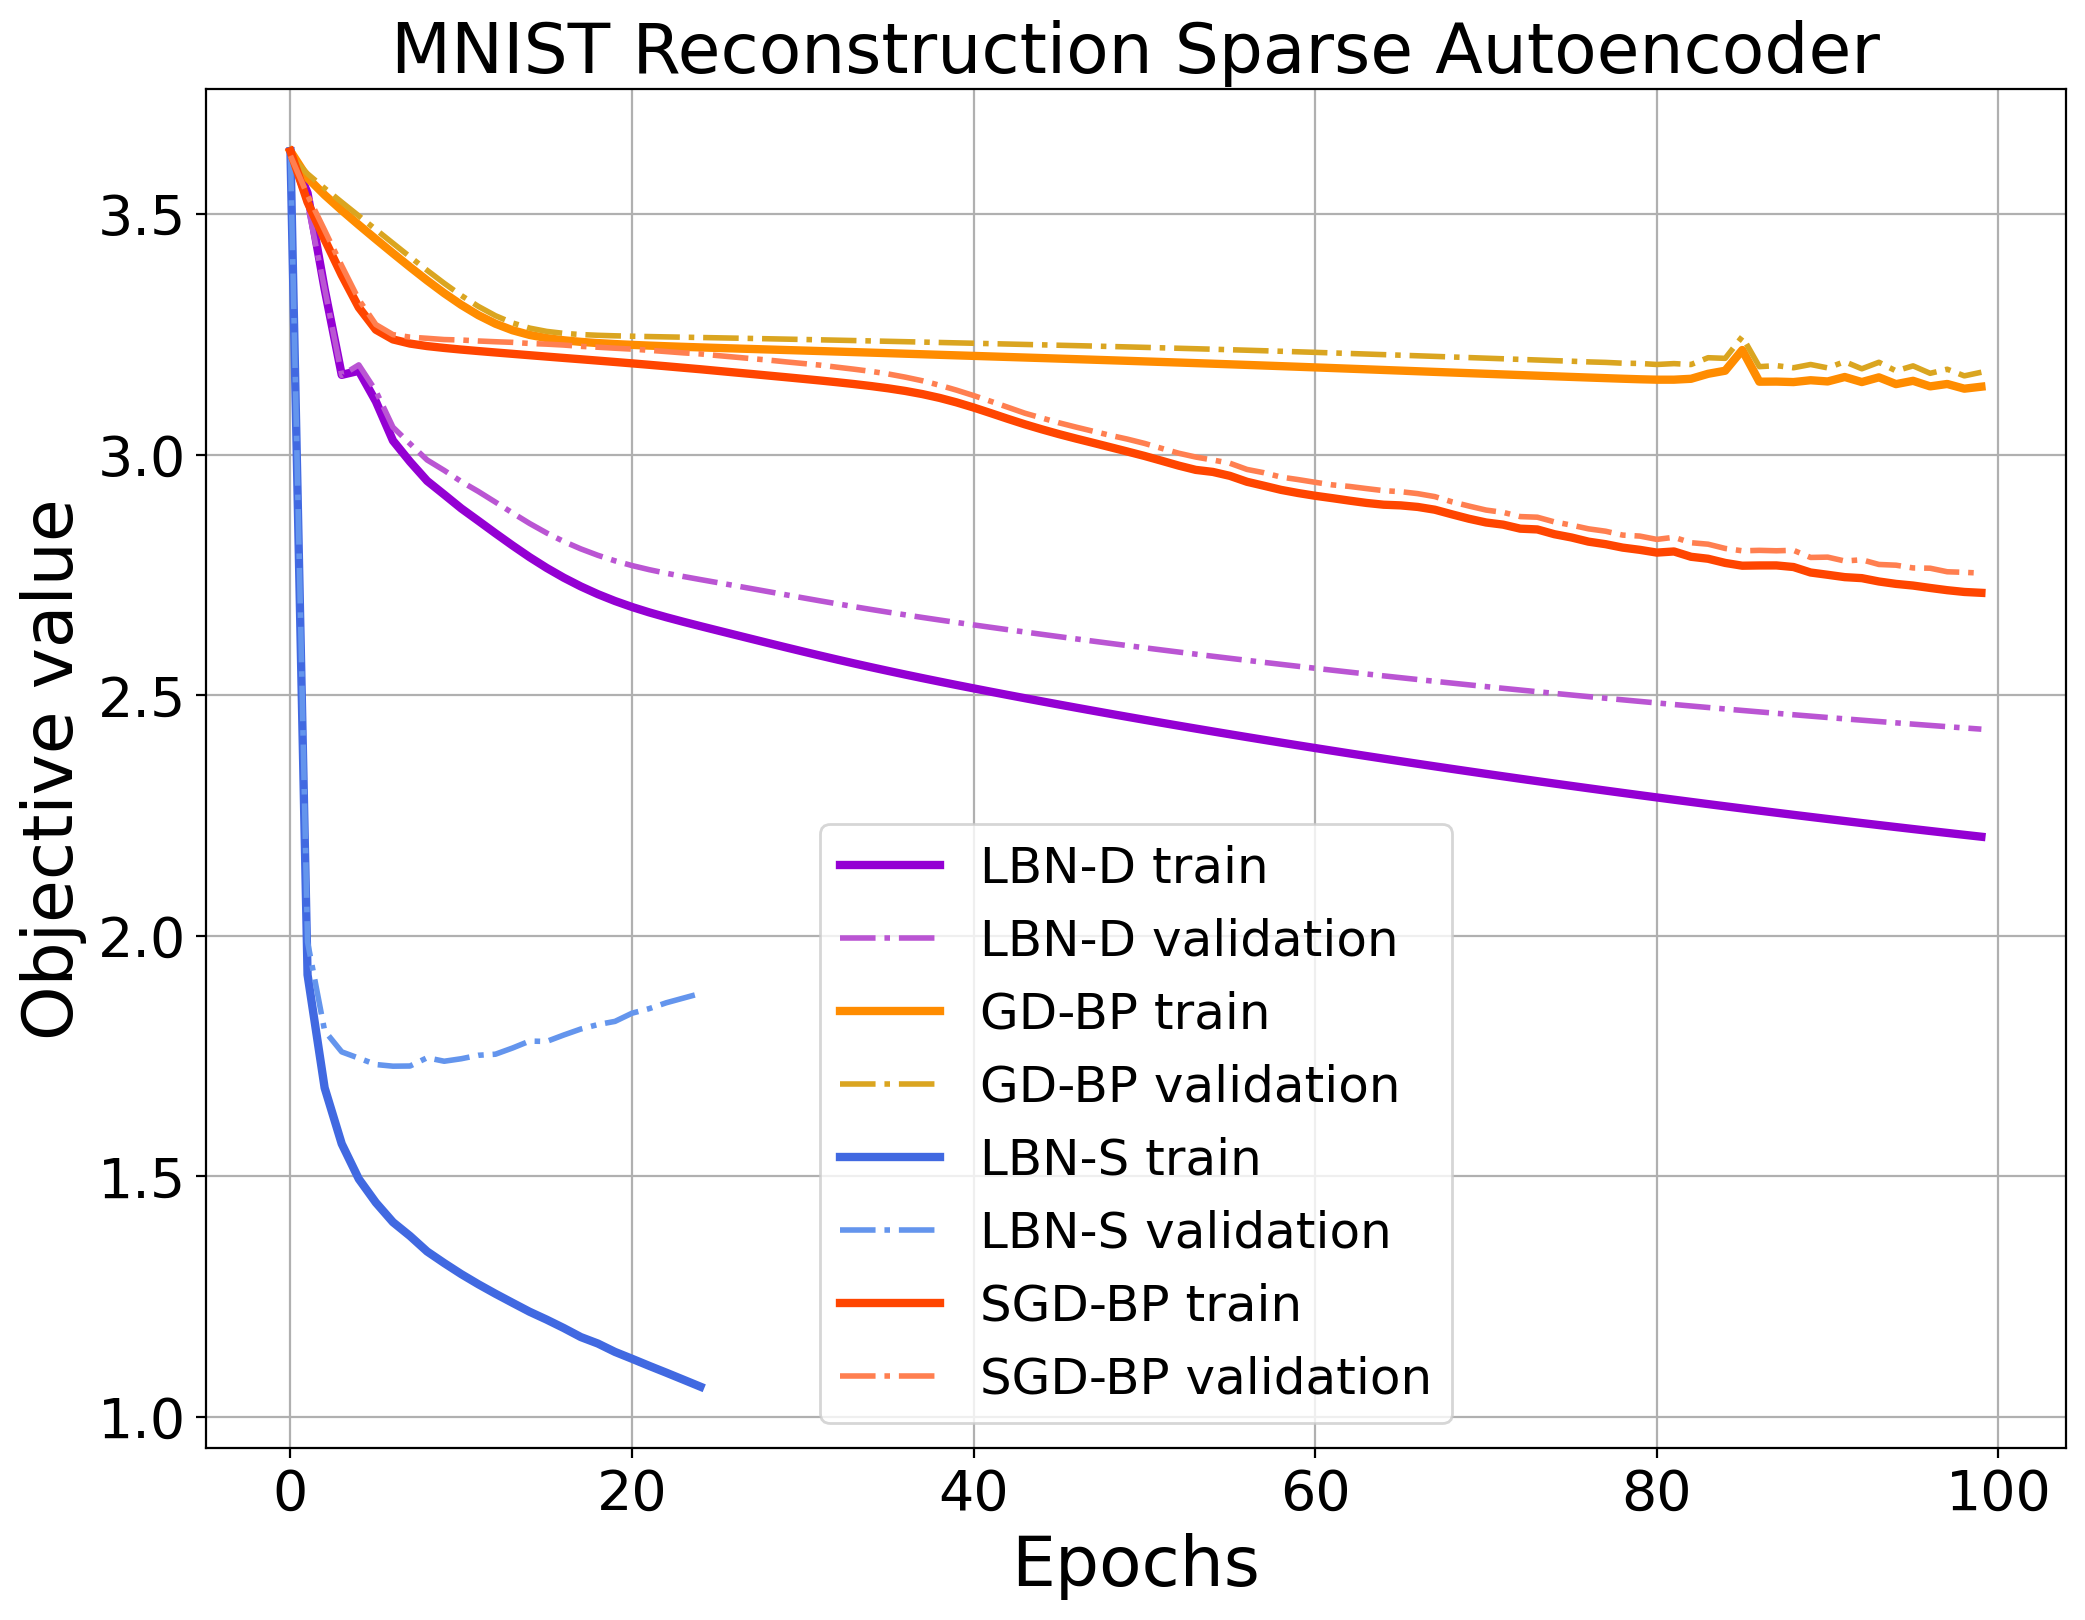
\includegraphics[width=0.88\linewidth]{lifted/Numerical_Recons_SAE_MNIST_objective_all_models.png}
        
        \column{0.48\textwidth}
        \centering
        \textbf{Validation Reconstructions} \\
        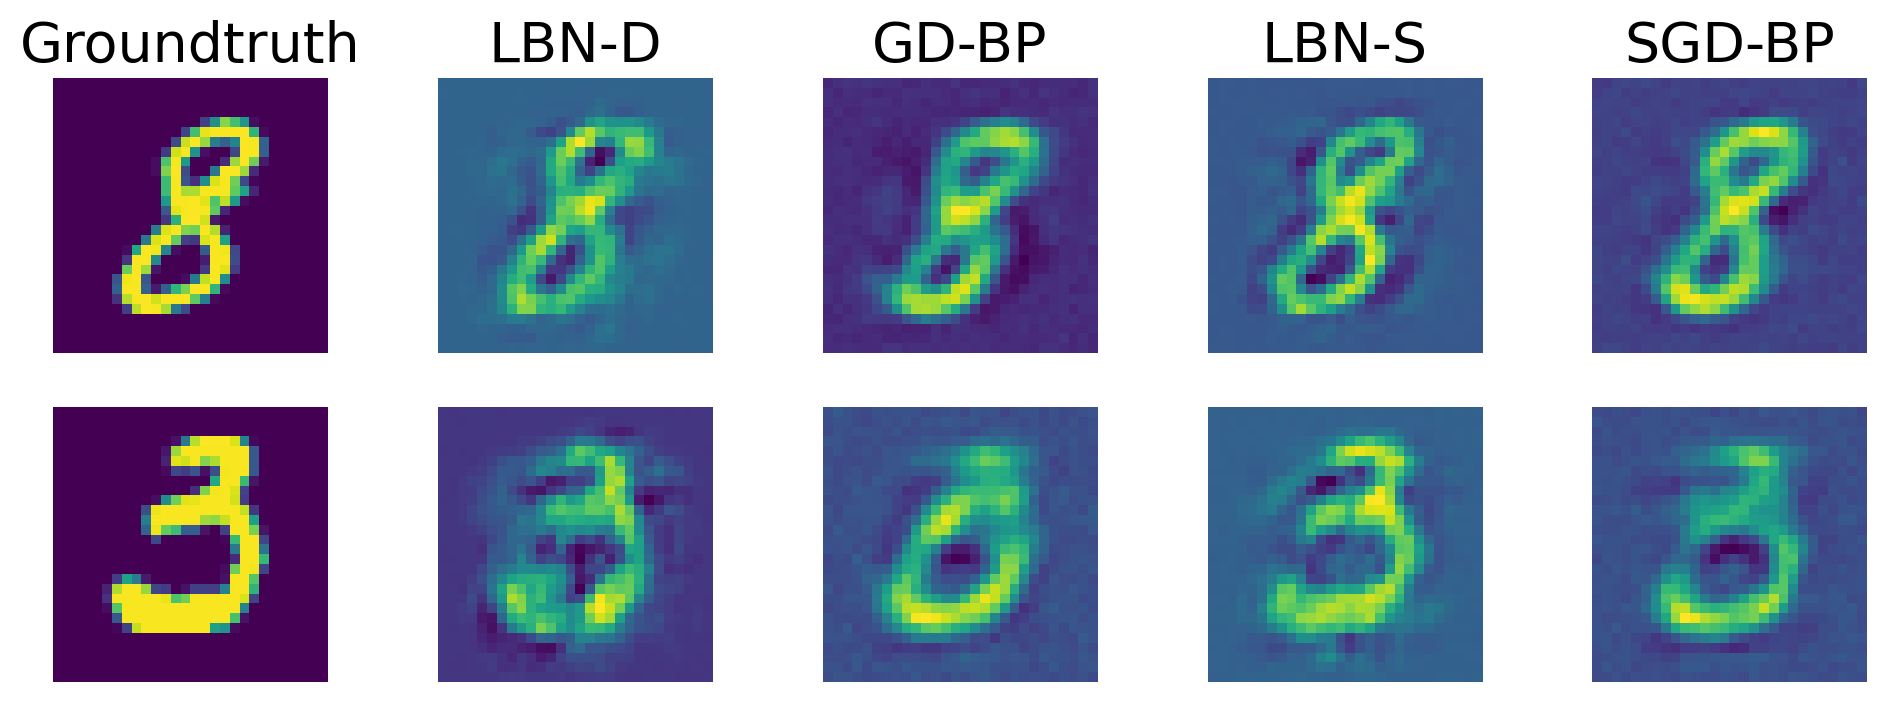
\includegraphics[width=\linewidth]{lifted/Numerical_Recons_SAE_MNIST_Recons_2_Val_Samples.png}
    \end{columns}
    
    \only<2->{\small Because $\alpha\|x_m^i\|_1$ is handled natively via a soft-thresholding block update on the variable $x_m^i$, the sparsity is enforced rigorously, unhindered by gradient propagation issues through the decoder.}
\end{frame}

\begin{frame}{Summary of Lecture 2}
    \begin{itemize}
        \item \textbf{Unified Framework:} The block-operator framework ($Au+d$, $Mu=Vz$, $z=\sigma(Wu+b)$) unifies perceptrons, MLPs, ResNets, and Unrolled Networks.
        \item \textbf{Penalty vs Architecture:} The difference between classical training and lifted training is merely swapping hard architectural constraints for soft Bregman relaxations.
        \item \textbf{Decoupled Solvers:} This formulation enables distributed Block-Coordinate Descent, allowing for inexact proximal updates (ISTA, ISGM) per layer.
        \item \textbf{Latent Control:} Explicit auxiliary variables allow for direct, rigorous regularisation of hidden layers (e.g., Sparse Autoencoders).
    \end{itemize}
    
    \textbf{Next Lecture:} We will reuse this exact same mathematical and algorithmic machinery to tackle the \textbf{stable inversion} of deep neural networks.
\end{frame}

\begin{frame}[allowframebreaks]{References}
    \bibliographystyle{abbrv}
    \bibliography{../../Lecture_Notes/references}
\end{frame}

\end{document}